\chapter{三相记忆的物理几何实现：从单体动力介质到多通路情景绑定体系}
本章我们讨论三相记忆的集中具体物理实现，用于加深对三相记忆原理的理解，并为后续工程实现提供参考。
\section{三相记忆首先是一种动力学结构，而不是存储设备分类}

此前已经将持续智能体的记忆系统抽象为三相结构
\[
\mathcal{M}_c=(h,E,\Theta),
\]
其中
\[
h=\mathrm{State},
\qquad
E=\mathrm{Trajectory},
\qquad
\Theta=\mathrm{Generator}.
\]

这里的三个变量并不首先对应三种具体存储器，而表示认知结构在不同时间尺度上的三种存在形式。工作记忆 $h$ 表示当前仍处于活跃状态的认知结构，情景记忆 $E$ 表示已经发生但仍以时间轨迹、事件关联或中期痕迹形式存在的经历结构，结构记忆 $\Theta$ 则表示已经通过长期巩固形成、能够重新生成和约束未来认知过程的慢结构。

因此三相记忆最基本的时间尺度关系为
\[
\tau_h \ll \tau_E \ll \tau_\Theta.
\]

传统数字系统可以分别用运行时激活、情景数据库和模型参数实现三者，但这并不是三相记忆的定义本身。更加一般地说，任何物理或计算系统，只要能够同时产生快状态、中期轨迹和慢结构，并且三者之间能够稳定发生双向转换，就原则上可以实现三相记忆。

因此三相记忆应首先被理解为
\[
\boxed{
\mathrm{State}
\leftrightarrow
\mathrm{Trajectory}
\leftrightarrow
\mathrm{Generator}
}
\]
这一多时间尺度动力学结构，而不是
\[
\mathrm{RAM}
+
\mathrm{Database}
+
\mathrm{ModelParameters}
\]
这一特定软件实现。

这一结论带来一个直接推论：如果未来计算介质本身能够具有连续状态、状态残留、可塑连接、吸引子结构以及多个特征时间尺度，那么三相记忆可以不再由传统数字计算机显式模拟，而由物理介质自身的动力学直接承载。

本章讨论两种代表性的物理实现路线。第一种是同一个连续动力介质内部同时承载 $h$、$E$ 与 $\Theta$；第二种则进一步进行功能分化，使当前语义、空间状态、情景绑定与长期生成结构由不同但耦合的物理区域共同实现。

\section{物理几何计算介质的抽象定义}

为了避免依赖某一种具体芯片，本章首先定义一种一般性的物理几何计算介质。设该系统由如下数学对象描述：
\[
\mathcal{G}
=
(
\mathcal{M},
g,
V,
\Gamma,
\boldsymbol{\tau}
).
\]

其中，$\mathcal{M}$ 表示系统能够访问的状态流形，$g$ 表示状态之间的有效距离、相似性或传播代价，$V$ 表示影响状态演化方向的有效势能景观，$\Gamma$ 表示不同局部状态单元之间的耦合拓扑，而 $\boldsymbol{\tau}$ 表示不同动力变量所对应的特征时间尺度集合。

这类系统与传统代数计算的关键区别在于，其计算不是完全由外部指令逐步规定，而允许系统状态根据其当前几何结构、局部耦合关系和外部输入自然演化。其一般形式可以写为
\[
dX
=
F(X,\Theta,u)\,dt
+
\Sigma(X,t)\,dW_t,
\]
其中 $X$ 表示当前快速状态，$\Theta$ 表示较慢的结构参数，$u$ 表示来自环境或高层系统的输入，$\Sigma dW_t$ 则表示可能存在的随机扰动。

后文使用 ``Geometric Computing Unit''，简称 GCU，指代一种按照上述原则构造的物理计算单元。这里的 GCU 不是本章理论成立的必要条件，而仅作为一种代表性工程实例。任何满足连续状态演化、状态残留和结构可塑性条件的物理介质，都可以被纳入同一分析框架。

从三相记忆角度看，关键并不在于器件采用忆阻、电磁振荡、光学传播、自旋电子学或其他技术，而在于物理系统能否形成
\[
\boxed{
\mathrm{FastState}
+
\mathrm{IntermediateTrace}
+
\mathrm{SlowStructure}
}
\]
三组清晰分离的时间尺度。

\section{单体物理介质中的三相记忆}

最简单的物理实现是不把三相记忆分散到三个独立模块，而是在同一个动力系统中为不同变量赋予不同时间常数。

设系统完整状态为
\[
X_G(t)
=
[
x(t),
m(t),
\Theta_G(t)
],
\]
其中 $x(t)$ 是快速运行状态，$m(t)$ 是中期残留状态，$\Theta_G(t)$ 是缓慢变化的长期结构。

这时可以建立最直接的三相映射：
\[
h(t)\equiv x(t),
\]
\[
E(t)\equiv m(t),
\]
\[
\Theta(t)\equiv \Theta_G(t).
\]

因此，同一个物理系统同时包含当前认知、经历痕迹和长期结构，只是这些状态存在于不同时间尺度上。

\section{工作记忆作为当前物理动力状态}

在这种实现中，工作记忆 $h(t)$ 不再首先意味着某段被显式寻址的存储空间，而是整个系统当前仍然处于活动状态的物理模式：
\[
\boxed{
h(t)=x(t).
}
\]

这些活动状态可以表现为局部场强、激活幅值、相位关系、频率同步、临时共振簇、短暂吸引子或其他能够在物理介质中维持有限时间的状态模式。

其一般动力学可以写成
\[
dx
=
F(x,m,\Theta_G,u)\,dt
+
\sqrt{2T(x,t)}\Sigma\,dW_t,
\]
其中 $T(x,t)$ 表示一个控制内部随机探索强度的有效动力学温度。这里的 ``温度'' 不必等于器件实际热力学温度，而是描述系统偏离当前吸引子并探索邻近状态空间的有效涨落强度。

当外部输入消失后，快速状态可以通过本征弛豫恢复：
\[
\tau_h \dot{x}
=
-x+F_{\mathrm{in}}.
\]
因此
\[
t\gg\tau_h
\]
时，某些当前激活会自然衰减，而不需要显式执行删除操作。

这提供了一种不同于地址式存储的工作记忆理解：
\[
\boxed{
\mathrm{WorkingMemory}
=
\mathrm{CurrentlySustainedDynamics}.
}
\]

换句话说，工作记忆不是一个地方，而是系统当前仍然在维持的状态。

\section{情景记忆作为中时间尺度残留}

如果一个系统只有快速状态 $x(t)$，那么任何状态一旦弛豫，过去经历便完全消失。因此需要引入比当前状态更慢的残留变量 $m(t)$。

其最简单动力学可以写成
\[
\tau_E \dot m
=
-m+
F_E(x),
\]
并要求
\[
\tau_E\gg\tau_h.
\]

于是，即使快速状态已经恢复到背景态，
\[
x(t+\Delta t)\approx x_{\mathrm{base}},
\]
过去的活动仍可能满足
\[
m(t+\Delta t)\neq 0.
\]

这种残留可以由多种物理机制承载，例如短时可塑电导、局部频率偏移、相位偏置、亚稳态、局部耦合暂时增强或其他中时间尺度状态变量。本章并不要求使用某一种特定器件。

从三相记忆角度看，过程
\[
h\rightarrow E
\]
被实现为
\[
\boxed{
\mathrm{FastState}
\rightarrow
\mathrm{PersistentTrace}.
}
\]

而召回
\[
E\rightarrow h
\]
则可以理解为过去残留改变当前动力学的有效势能，使曾经出现过的状态更加容易重新激活。例如
\[
m
\rightarrow
V_{\mathrm{eff}}
\rightarrow
x.
\]

因此，物理系统中的召回不一定需要显式搜索某个地址，而可以表现为
\[
\boxed{
\mathrm{PastTrace}
\rightarrow
\mathrm{AttractorReactivation}.
}
\]

必须特别注意，这里所得到的首先是中期经历痕迹，而不是已经完成完整语义绑定的情景记忆。简单的残留变量能够说明“某种状态曾经发生”，但尚不足以表示“什么对象在什么地点、什么时间发生了什么关系”。这一限制将在后文成为引入专门情景绑定系统的直接原因。

\section{结构记忆作为慢几何结构}

长期结构记忆 $\Theta$ 不能依赖持续高强度激活，否则系统将同时面临能耗和稳定性问题。更加自然的实现，是让反复出现的稳定关系逐渐改变系统自身较慢的结构参数。

将这些长期参数统一记为
\[
\Theta_G
=
\{
W_{ij},
g_{ij},
\omega_i,
K_{ij},
\tau_i,
V,
\Gamma,
\ldots
\}.
\]

其中，$W_{ij}$ 可以表示局部有效连接强度，$g_{ij}$ 表示状态之间的有效几何关系，$\omega_i$ 表示本征动力时间或振荡频率，$K_{ij}$ 表示耦合强度，$\tau_i$ 表示局部时间常数，$V$ 表示势能结构，而 $\Gamma$ 表示整体功能拓扑。

简单的局部连接变化可以写为
\[
\dot W_{ij}
=
\eta m_i m_j
-
\lambda W_{ij},
\]
但更一般的结构学习应表示为
\[
\boxed{
\dot\Theta_G
=
P(
x,
m,
\varepsilon,
T,
v,
\Theta_G
),
}
\]
其中 $\varepsilon$ 表示预测残差，$T$ 表示探索强度，$v$ 表示价值或重要度调制，而 $P$ 表示受到安全、稳定性和物理约束的长期可塑性规则。

由此
\[
E\rightarrow\Theta
\]
获得明确物理意义：
\[
\boxed{
\mathrm{RepeatedTrajectory}
\rightarrow
\mathrm{SlowGeometry}.
}
\]

长期学习不是永久保持过去所有瞬时状态，而是让反复出现的有效关系逐渐成为以后状态演化的结构条件。这一过程可以概括为
\[
\boxed{
\mathrm{HistoryBecomesStructure}.
}
\]

\begin{figure}[htbp]
\centering
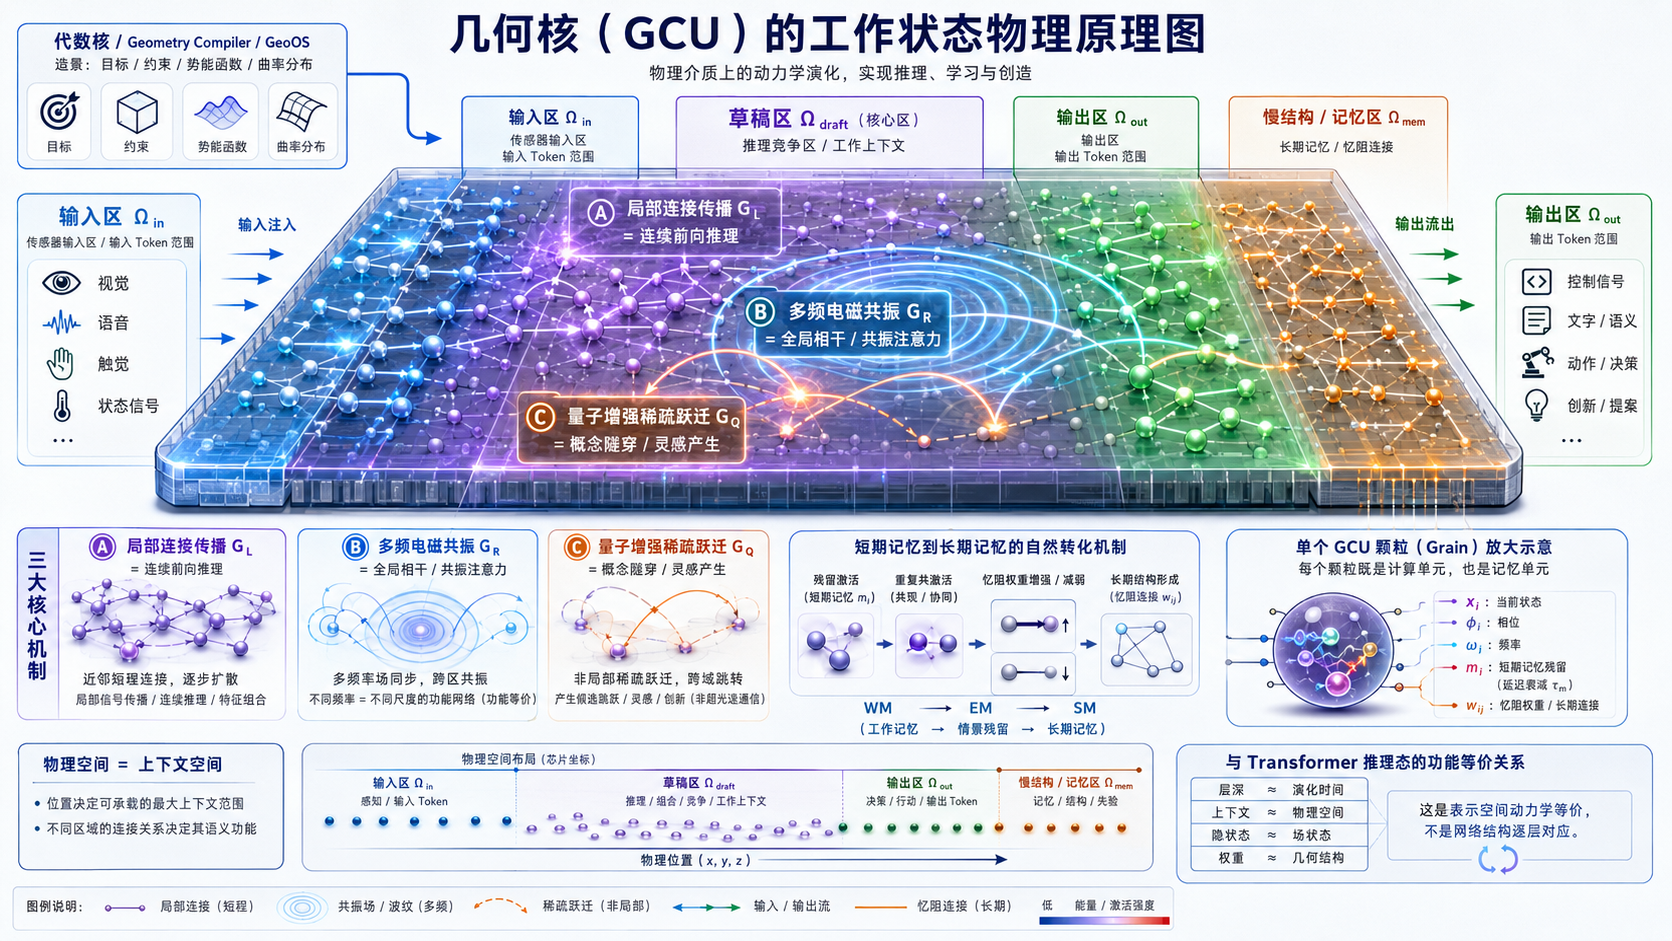
\includegraphics[width=.9\textwidth,height=.40\textheight,keepaspectratio]{images/GCU.png}
\caption{GCU的物理架构实现三相记忆动力学}
\end{figure}


\section{单体三相记忆的快--慢动力系统}

单体物理实现可以统一写成如下多时间尺度系统：
\[
dx
=
F(x,m,\Theta_G,u,T)\,dt
+
\Sigma\,dW_t,
\]
\[
\tau_E\dot m
=
G(x,m),
\]
\[
\tau_\Theta\dot\Theta_G
=
P(x,m,\Theta_G,\varepsilon,v),
\]
其中
\[
\tau_h
\ll
\tau_E
\ll
\tau_\Theta.
\]

于是三相关系表现为
\[
x
\leftrightarrow
m
\leftrightarrow
\Theta_G.
\]

其中
\[
x\rightarrow m
\]
表示当前活动形成经历痕迹，
\[
m\rightarrow x
\]
表示过去痕迹重新影响当前状态，
\[
m\rightarrow\Theta_G
\]
表示经历的长期巩固，
\[
\Theta_G\rightarrow x
\]
则表示慢结构直接塑造快速活动。

因此，三相记忆不是简单的单向
\[
h\rightarrow E\rightarrow\Theta,
\]
而是一个完整的双向快--慢动力体系：
\[
\boxed{
h
\leftrightarrow
E
\leftrightarrow
\Theta.
}
\]

从这一视角看，记忆并不是被 ``存入'' 一个系统，而是同一个认知结构逐渐进入更慢的动力尺度。

\section{单体实现的理论优势与边界}

单体物理实现的主要优势在于计算与记忆不再严格分离。当前思维、经历痕迹和长期结构可以存在于同一个介质内：
\[
\mathrm{Computation}
+
\mathrm{WorkingMemory}
+
\mathrm{ExperienceTrace}
+
\mathrm{StructuralMemory}
\]
成为同一动力系统的不同时间尺度。

这与此前提出的智能频谱理论一致：
\[
\boxed{
\mathrm{SameSystem},
\mathrm{DifferentTimescales}.
}
\]

同时，它也为认知结构迁移提供了直接物理解释：
\[
\boxed{
\mathrm{FastActivity}
\rightarrow
\mathrm{SlowStructure}.
}
\]

但是这种实现存在重要边界。一般的中期残留
\[
m(t)
\]
只能说明过去状态在系统中留下痕迹，却不能自动产生完整的情景对象
\[
E_i
=
(
\mathrm{what},
\mathrm{where},
\mathrm{when},
\mathrm{relation},
\ldots
).
\]

因此必须严格区分
\[
\boxed{
\mathrm{PersistentTrace}
\neq
\mathrm{StructuredEpisode}.
}
\]

当 Agent 开始进入复杂具身环境时，真正需要回答的问题不再只是“此前激活过什么”，而是
\[
\boxed{
\mathrm{What\ happened,\ where,\ when,\ and\ in\ relation\ to\ whom?}
}
\]

这使三相记忆从同质动力实现进一步走向功能分化。

\section{双通路表示：为什么必须区分 What 与 Where}

具身智能中的一个基本结构是，对象的语义身份与对象在当前世界中的空间状态并非同一种信息。

为此可以定义两个相对独立但持续耦合的表示空间：
\[
\Omega_W
\]
与
\[
\Omega_S.
\]

其中 $\Omega_W$ 表示语义对象空间，主要回答
\[
\mathrm{What\ is\ it?}
\]
例如类别、属性、功能、对象身份和概念关系。

$\Omega_S$ 表示空间--行动状态空间，主要回答
\[
\mathrm{Where\ is\ it?}
\qquad
\mathrm{How\ can\ I\ interact\ with\ it?}
\]
例如位置、方向、距离、运动轨迹、身体坐标和可达性。

其当前状态分别记为
\[
X_W(t),
\qquad
X_S(t).
\]

这种分离的主要意义不是简单模仿生物视觉通路，而是避免把对象身份与每一个具体空间位置过早融合。例如同一个杯子可以先形成稳定语义表示
\[
C_{\mathrm{cup}},
\]
再分别与
\[
S_{\mathrm{kitchen}},
\quad
S_{\mathrm{bedroom}},
\quad
S_{\mathrm{table}}
\]
建立不同关系。

于是对象本身可以保持稳定，而对象--位置关系作为独立结构动态变化。

这可以概括为
\[
\boxed{
\mathrm{StableIdentity}
+
\mathrm{VariableSituation}
}
\]
的分离。

后文使用 ``What-GCU'' 和 ``Where-GCU'' 分别指代实现这两个空间的候选物理几何计算区域。它们仍然只是工程实例，理论本身并不要求特定器件。

\section{为什么双通路仍然不足以形成情景记忆}

只有
\[
X_W(t)
\]
和
\[
X_S(t)
\]
仍然无法得到完整情景，因为系统还需要记住：

某个对象在什么时间位于什么位置；

谁与该对象发生了什么动作；

这些关系是否与当前主体有关；

该事件后来产生了什么结果。

因此必须增加一个新的功能：
\[
\boxed{
\mathrm{Binding}.
}
\]

这里的 Binding 不是简单拼接两个向量，而是产生一个可以被再次寻址、模式补全和重新激活的关系结构。

因此定义情景绑定算子
\[
B:
(
W,S,T,R,A,V
)
\rightarrow
E_i,
\]
其中 $W$ 表示 What 状态，$S$ 表示 Where 状态，$T$ 表示时间结构，$R$ 表示关系，$A$ 表示动作或事件，而 $V$ 表示价值或重要度调制。

于是
\[
\boxed{
E_i
=
B(W_i,S_i,T_i,R_i,A_i,V_i)
}
\]
形成一个真正意义上的情景结构。

\section{海马式几何绑定单元的抽象定义}

为了实现上述 Binding，可引入一个专门的情景关系绑定系统。后文称其为
\[
\mathrm{HGU}
=
\mathrm{Hippocampal\ Geometric\ Unit},
\]
即海马式几何绑定单元。

这里 ``海马式'' 只表示功能上的设计借鉴：快速建立事件索引、关系绑定、模式补全以及从部分线索重新激活相关分布式表示。它并不意味着硬件必须复制生物海马的解剖结构。

HGU 的理论角色不是传统数据库，而是
\[
\boxed{
\mathrm{DynamicRelationalBinder}.
}
\]

因此 What 区域主要承载
\[
\text{对象是什么},
\]
Where 区域主要承载
\[
\text{对象在哪里},
\]
而 HGU 主要承载
\[
\boxed{
\text{这个对象在这个时间、这个地点发生了什么关系}.
}
\]

例如一个事件可以抽象表示为
\[
E_i=
(
\mathrm{blue\ cup},
\mathrm{kitchen\ table},
20{:}00,
\mathrm{owner},
\mathrm{placing}
).
\]

这里被保存的核心不是重复复制 ``cup'' 的全部语义结构，而是建立
\[
\mathrm{Cup}
\leftrightarrow
\mathrm{Kitchen}
\leftrightarrow
\mathrm{Time}
\leftrightarrow
\mathrm{Action}
\]
之间的一次具体关系实例。

\section{多区域体系下工作记忆的重新定义}

当 What、Where 和 HGU 等多个区域同时存在后，工作记忆 $h$ 不再合理地对应单一硬件区域。

更加一般的形式是
\[
\boxed{
h(t)
=
[
X_W(t),
X_S(t),
X_H^{\mathrm{active}}(t),
X_C(t)
],
}
\]
其中 $X_H^{\mathrm{active}}$ 表示当前被激活的情景索引或绑定结构，$X_C$ 表示当前控制、目标和其他参与显式认知的活动状态。

因此工作记忆更准确地定义为
\[
\boxed{
h=
\mathrm{TemporarilyCoherentDistributedState}.
}
\]

也就是说，工作记忆并不一定是所有信息被物理搬运到一个中心，而可以是一组分布在不同功能区域、但在当前时刻形成临时高耦合或同步关系的活动结构。

这一物理解释与此前的
\[
\boxed{
h=
\mathrm{SparseExplicitCrossScaleSurface}
}
\]
保持一致：只有当前真正需要跨功能全局协调的 Agent-CSO 才进入这一临时协同状态，而绝大多数低层动力过程仍然局部闭合。

\section{HGU 中的情景形成与模式补全}

当一个当前经历满足足够的新颖性、价值性、预测误差、目标相关性或自我相关性时，系统可以触发
\[
\mathrm{EpisodeFormation}.
\]

HGU 接收
\[
W_t,\quad
S_t,\quad
T_t,\quad
R_t,\quad
A_t
\]
并形成
\[
\boxed{
E_i=B(W_t,S_t,T_t,R_t,A_t).
}
\]

这一情景结构可以在内部形成一个稳定或亚稳定吸引子
\[
\mathcal{A}_{E_i}.
\]

在未来，只需要一个不完整线索，例如
\[
\mathrm{Cup}
\]
或
\[
\mathrm{Kitchen},
\]
便可能触发
\[
\mathrm{Cue}
\rightarrow
HGU
\rightarrow
E_i
\rightarrow
\mathrm{What/Where\ Reactivation}.
\]

因此情景召回
\[
E\rightarrow h
\]
获得一种明确的物理实现：
\[
\boxed{
\mathrm{PartialCue}
\rightarrow
\mathrm{EpisodeAttractor}
\rightarrow
\mathrm{DistributedPatternCompletion}.
}
\]

这里的关键不是 ``查找一条记录''，而是利用绑定结构恢复此前共同出现的多个状态空间。

\begin{figure}[htbp]
\centering
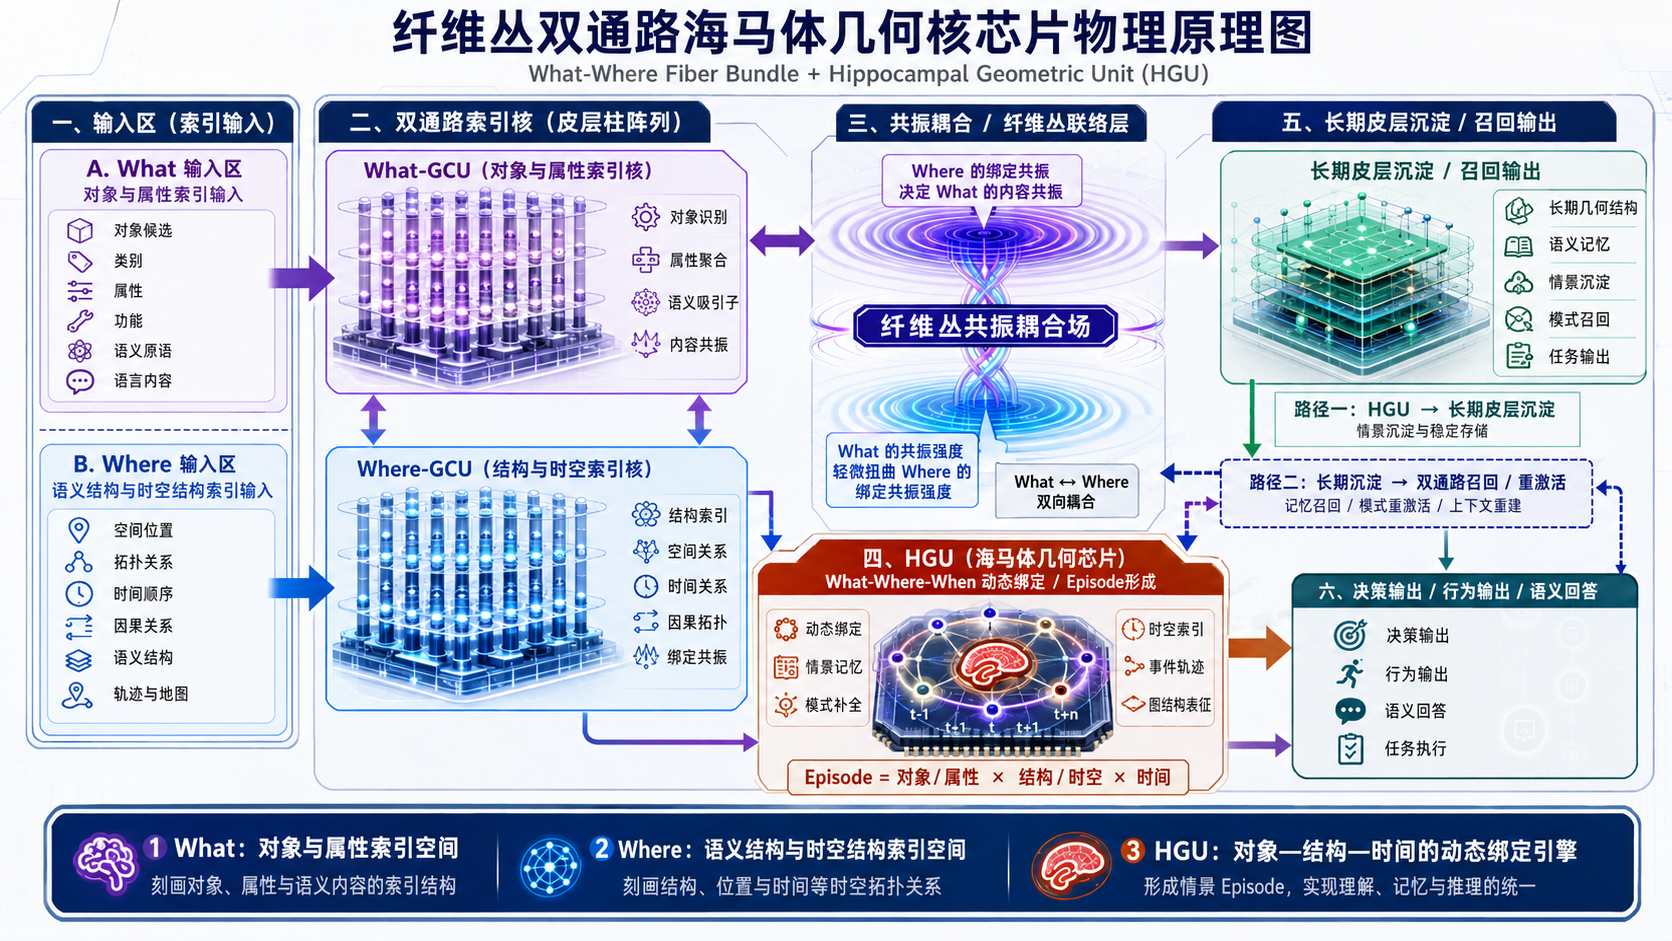
\includegraphics[width=.9\textwidth,height=.40\textheight,keepaspectratio]{images/HCU.png}
\caption{双通路GCU实现三相记忆动力学}
\end{figure}

\section{从情景到结构：E 到 Theta 的长期巩固}

单个 Episode 不应直接成为世界长期结构。否则一次偶然事件就可能永久改变 Agent 的世界模型。

因此
\[
E\rightarrow\Theta
\]
必须依赖重复、稳定性和现实验证。

设经历集合为
\[
\{E_1,E_2,\ldots,E_n\}.
\]
若其中反复出现某些稳定关系，则可逐渐形成
\[
\boxed{
\mathrm{RepeatedEpisodeRelations}
\rightarrow
\mathrm{StableGenerativeGeometry}.
}
\]

例如，大量不同事件可能共同支持
\[
\mathrm{Cup}
\leftrightarrow
\mathrm{Kitchen},
\]
或者
\[
\mathrm{SpecificPerson}
\leftrightarrow
\mathrm{RepeatedRoutine}.
\]

这些跨情景稳定结构不再依赖某一单次 Episode，而被压缩进更慢的语义、空间、因果或技能结构中。

因此可以把 HGU 和长期几何区域的功能差异抽象为
\[
\boxed{
\mathrm{EpisodeSystem}
:
\mathrm{Fast,\ Sparse,\ InstanceSpecific},
}
\]
\[
\boxed{
\mathrm{StructuralSystem}
:
\mathrm{Slow,\ Distributed,\ Statistical,\ Generative}.
}
\]

这种快情景--慢结构分工与互补学习系统思想具有明显对应，但本章将其推广为一种硬件无关的三相记忆实现原则。

\section{结构记忆如何重新解释情景记忆}

三相记忆不是单向巩固过程。新的长期结构也会改变旧经历的意义。

设过去存在事件
\[
E_i.
\]
随着后续学习，长期结构从
\[
\Theta
\]
变化为
\[
\Theta'.
\]

同一事件可以得到新的解释：
\[
\boxed{
E_i'
=
\mathrm{Interpret}(E_i,\Theta').
}
\]

因此，理想的 HGU 不必永久冻结一个完整语言叙事，而可以保存
\[
\boxed{
\mathrm{EpisodeIndex}
+
\mathrm{RelationalTrace}
}
\]
并在召回时利用当前 $\Theta$ 重建具体语义。

这样
\[
\Theta\rightarrow E
\]
就表现为
\[
\boxed{
\mathrm{CurrentGenerativeStructure}
\rightarrow
\mathrm{ReinterpretationOfPastExperience}.
}
\]

这一机制十分重要，因为持续智能体对同一人生经历的理解会随着知识、自我和价值结构发展而变化。

\section{慢结构如何塑造当前认知}

长期结构
\[
\Theta
\]
的核心作用并不是静态存储，而是改变未来状态演化。

设当前状态满足
\[
\dot x
=
-\nabla V_\Theta(x)
+
F_{\mathrm{interaction}}.
\]

这里 $V_\Theta$ 由长期结构决定，因此每一个新输入都不是在空白空间中被重新计算，而是在已经被历史经历塑形的动力景观中继续演化。

这意味着
\[
\Theta\rightarrow h
\]
在物理实现中等价于
\[
\boxed{
\mathrm{SlowGeometry}
\rightarrow
\mathrm{FastDynamics}.
}
\]

这一关系正是全书多时间尺度理论的核心：
\[
\boxed{
\mathrm{SlowStructureShapesFastActivity}.
}
\]

\section{为什么从当前状态直接修改长期结构必须受到严格限制}

理论上三相记忆允许
\[
h\rightarrow\Theta
\]
的快速修正，但在物理可塑系统中必须严格限制这一路径。

如果每一个瞬时异常状态都直接改变长期几何结构，就可能导致偶然噪声固化、错误世界模型形成、结构漂移以及对抗性污染。

因此更安全的默认路径应为
\[
\boxed{
h
\rightarrow
\mathrm{TemporaryTrace}
\rightarrow
E
\rightarrow
\mathrm{Validation}
\rightarrow
\Theta.
}
\]

只有满足极高置信度、强监督或特殊安全条件的结构，才允许使用较快的
\[
h\rightarrow\Theta
\]
通道。

这实际上是此前
\[
\boxed{
\mathrm{SlowVariableProtection}
}
\]
原则在物理记忆系统中的具体实现。

\section{自我、价值与情景写入}

完整 Agent 的情景记忆不应等价于世界的客观录像。智能体必须根据自身价值、自我关系和长期目标决定哪些事件真正值得进入长期经历结构。

设 Episode 写入概率为
\[
P(E_i\;\mathrm{write})
=
\sigma
\left(
\alpha N_i
+
\beta V_i
+
\gamma G_i
+
\delta S_i
+
\eta\varepsilon_i
\right),
\]
其中 $N_i$ 表示新颖性，$V_i$ 表示价值或内稳态重要性，$G_i$ 表示目标相关度，$S_i$ 表示自我相关度，而 $\varepsilon_i$ 表示预测残差。

此前 AgentOS 中定义的慢自我结构 $\Psi$ 在这里并不是另一块情景存储器，而主要影响
\[
\boxed{
\mathrm{WhichEventsBecomeMyEpisodes}.
}
\]

同样，AHC 或身体影响状态可以给情景附加功能性调制标签，使以后召回的不仅是
\[
\mathrm{What}
+
\mathrm{Where}
+
\mathrm{When},
\]
还包括
\[
\mathrm{HowThisEventAffectedTheAgent}.
\]

因此可以把一个更完整的情景写成
\[
E_i
=
(
W_i,
S_i,
T_i,
R_i,
A_i,
F_i
),
\]
其中 $F_i$ 是与该事件相关的身体或功能影响摘要，而不是完整复制整个身体场状态。

\section{生命周期吸引子与物理记忆系统}

在 AgentOS 中，$\Psi$ 表示长期身份与价值结构，而更慢的 $\Omega$ 或 DGA 表示生命周期尺度的生成吸引子，即系统 ``正在成为怎样的主体''。

因此
\[
\tau_\Omega\gg\tau_\Theta.
\]

在物理实现中，不应简单把 $\Omega$ 映射成某个固定存储单元。更合理的理解是让其影响：

\begin{itemize}
    \item 哪些结构具有更高的长期可塑性；
    \item 哪些吸引子族具有更高的长期增益；
    \item 哪些目标结构长期受到偏置；
    \item 哪些区域允许改变、哪些区域受到保护；
    \item 哪些经历更容易进入长期结构。
\end{itemize}

因此可以抽象为
\[
\boxed{
\Omega
\rightarrow
\mathrm{PlasticityLandscape}.
}
\]

从这一视角看，$\Theta$ 更接近 ``我已经学会什么''，而 $\Omega$ 更接近 ``我的长期结构朝什么方向允许继续改变''。

\section{What--Where 表示系统与 SGC 的关系}

此前 AgentOS 工程中定义了
\[
\mathrm{SGC}
=
\mathrm{SemanticGraphCoordinateSpace},
\]
即主体当前可行动现实的显式语义图坐标空间。SGC 需要包含对象、位置、关系、属性、可行动性以及认识论状态，并且必须能够被 Agent Kernel 和工程人员检查。

因此 Where 物理动力区域不能直接等同于 SGC：
\[
\boxed{
\mathrm{WherePhysicalSpace}
\neq
\mathrm{SGC}.
}
\]

前者可以拥有大量面向高速计算的私有物理状态，而 SGC 是对这些状态经过语义化后的公开 ABI。

更加合理的关系为
\[
\mathrm{WhereSystem}
\xrightarrow{\mathrm{Decoder}}
\mathrm{SGC}.
\]

What 表示系统则向 SGC 提供对象身份、语义属性和关系候选。因此整体可写为
\[
\boxed{
\mathrm{WhatSystem}
+
\mathrm{WhereSystem}
\rightarrow
\mathrm{SGC}.
}
\]

HGU 则进一步提供过去的 What--Where--When 关系，使当前 SGC 获得持续实体身份、历史关系和情景上下文。

因此
\[
\boxed{
\mathrm{CurrentObservation}
+
\mathrm{EpisodicContext}
\rightarrow
\mathrm{SGC}_t.
}
\]

\section{情景记忆与 FCS/AHC 的关系}

SGC 主要回答现实中 ``有什么、在哪里、与谁有关''，而此前定义的 FCS 则描述当前现实和身体状态如何功能性影响主体。

因此 Episode 的形成不能只读取 What 与 Where，也应从 FCS/AHC 中提取与事件有关的低维影响摘要。

例如某一事件可能携带
\[
F_i=
(
\mathrm{Threat},
\mathrm{Urgency},
\mathrm{Arousal},
\mathrm{EnergyImpact},
\ldots
).
\]

当该 Episode 被重新激活时，这一影响摘要可以重新进入 AHC，使过去经历对当前控制产生适当的调制作用。

需要强调的是
\[
\boxed{
\mathrm{EpisodeAffectTag}
\neq
\mathrm{CompleteFCSReplay}.
}
\]

情景记忆只保存与事件相关的功能影响，而不是逐帧复制当时全部身体状态。

\section{单体实现与多通路实现的统一关系}

单体物理系统与 What--Where--HGU 多通路系统并不是两套互相排斥的理论，而是同一三相记忆原理的不同功能分化程度。

单体方案可以写为
\[
h=x,
\qquad
E=m,
\qquad
\Theta=\Theta_G.
\]

多通路方案则可以写成
\[
h=
[
X_W,
X_S,
X_H^{\mathrm{active}},
X_C
],
\]
\[
E=
\{E_i\}_{\mathrm{binder}},
\]
\[
\Theta=
[
\Theta_W,
\Theta_S,
\Theta_R,
\Theta_{\mathrm{skill}},
\ldots
].
\]

因此二者关系可以概括为
\[
\boxed{
\mathrm{HomogeneousMemoryDynamics}
\rightarrow
\mathrm{FunctionallyDifferentiatedMemorySystem}.
}
\]

系统规模较小时，同一个物理介质可以同时承担当前状态、经历残留和长期结构；当情景绑定、空间导航、概念泛化和长期巩固成为稳定且高频的独立需求时，系统可能出现专门化功能区域。

这与前文定义
\[
\boxed{
\mathrm{Module}
=
\mathrm{StableTopologicalCondensate}
}
\]
完全一致：所谓专用情景绑定器，不必在理论上被规定为从系统诞生时便存在，而可以被理解为长期稳定功能需求形成的拓扑凝聚。

\section{三相记忆实现的 CSO 无关性}

从 CSO 理论看，三相记忆的不同硬件实现进一步证明了 ``本体结构'' 与 ``承载结构'' 必须分离。

设某个情景本体为
\[
C_{\mathrm{episode}}.
\]

在单体介质中，它可能实现为
\[
\pi_1(C_{\mathrm{episode}})
=
\mathrm{DistributedMetastablePattern}.
\]

在专门情景绑定架构中，它可能实现为
\[
\pi_2(C_{\mathrm{episode}})
=
\mathrm{BindingAttractor}.
\]

虽然
\[
\pi_1(C)\neq\pi_2(C),
\]
但两者可能仍然承载同一个认知本体：
\[
\boxed{
\mathrm{Ontology}[\pi_1(C)]
=
\mathrm{Ontology}[\pi_2(C)]
=
C.
}
\]

因此
\[
\boxed{
\mathrm{SameCSO}
\neq
\mathrm{SameCarrier}.
}
\]

这也是为什么三相记忆不能由某一种数据库、网络参数或芯片器件来定义。

\section{三相记忆与结构频谱迁移}

物理实现使三相记忆与此前的认知结构频谱理论获得直接联系。

设
\[
\rho_{\mathrm{CSO}}(f,\omega,t)
\]
表示 Agent-CSO 在功能位置 $f$ 和时间频率 $\omega$ 上的分布。

则工作态主要占据较快时间尺度
\[
\omega_h,
\]
情景轨迹占据中间尺度
\[
\omega_E,
\]
结构记忆主要占据更慢尺度
\[
\omega_\Theta.
\]

因此记忆巩固可以重新写成
\[
\boxed{
\mathrm{MemoryConsolidation}
=
\mathrm{CSOSpectralMigration}.
}
\]

即
\[
\boxed{
\mathrm{FastActiveCSO}
\rightarrow
\mathrm{IntermediateEpisodeCSO}
\rightarrow
\mathrm{SlowGenerativeCSO}.
}
\]

这里真正迁移的不是一份完整数据从一个地址复制到另一个地址，而是同一相关认知结构逐步获得更长时间常数、更稳定承载和更低运行成本。

\section{认知温度与结构学习必须严格分离}

物理动力系统可以通过增加随机扰动强度扩大状态搜索。用有效温度 $T$ 表示时，吸引子逃逸概率可以近似具有
\[
P_{\mathrm{escape}}
\propto
\exp\left(
-\frac{\Delta V}{T}
\right)
\]
形式。

但是必须严格区分
\[
\boxed{
\mathrm{Exploration}
\neq
\mathrm{Learning}.
}
\]

升高 $T$ 只是让系统访问更多候选状态，并不意味着这些候选状态都应该进入慢结构。

因此合理时序应是
\[
\boxed{
\mathrm{TemperatureRise}
\rightarrow
\mathrm{StateExploration}
\rightarrow
\mathrm{CandidateDiscovery}
\rightarrow
\mathrm{Verification}
\rightarrow
\mathrm{EpisodeFormation}
\rightarrow
\mathrm{SlowConsolidation}.
}
\]

不能简单采用
\[
T\uparrow
\Rightarrow
\Theta\ \mathrm{changes}.
\]

这一原则实际上与 AgentOS 中 TCE 的设计一致。TCE 控制的是系统 ``以怎样的动力状态进行认知''，而不是直接决定 ``什么必须被写成长期知识''。

\section{物理动力调制与 TCE 的接口}

TCE 是 AgentOS 中用于调节认知温度、探索程度、注意增益、抑制和认知稳定度的控制器。

如果底层采用物理动力介质，那么 TCE 的部分抽象控制量可以映射为真实物理调制：
\[
u_{\mathrm{TCE}}
\rightarrow
[
T(x,t),
G(x,t),
I(x,t),
R(x,t)
],
\]
其中 $T$ 表示有效认知温度，$G$ 表示增益场，$I$ 表示抑制场，而 $R$ 表示共振或局部传播偏置。

于是产生
\[
\boxed{
\mathrm{SoftwareCognitiveControl}
\rightarrow
\mathrm{PhysicalDynamicalModulation}.
}
\]

这并不意味着 TCE 必须由某个特定 NPU 实现。TCE 是功能概念，而 CPU、NPU、模拟控制电路、GCU 内部调制器都可能承载其中不同部分。

因此必须坚持
\[
\boxed{
\mathrm{FunctionalOntology}
\neq
\mathrm{HardwarePlacement}.
}
\]

\section{稳定几何、软件孪生与可塑几何}

为了进一步区分训练、稳定运行和终身结构学习，可以定义三种同一几何动力系统的实现状态。

第一种是软件动力孪生体，用于在传统计算设备上模拟完整物理动力学、训练结构参数、分析噪声和验证稳定性。后文可简称为 GCU-S。

第二种是稳定物理实现体，其长期几何结构在正常在线运行过程中受到保护，主要执行当前动力学和有限短时记忆。后文可简称为 GCU-H。

第三种是具有长期结构可塑性的物理实现体，即允许
\[
\dot\Theta_G\neq 0
\]
的终身学习版本。后文可简称为 GCU-L。

三者不是三种不同的三相记忆理论，而是同一理论的不同可塑性配置。

对稳定实现体而言，
\[
\Theta_G\approx\mathrm{const}
\]
在正常任务期间成立，但仍然允许
\[
h
\leftrightarrow
E
\]
快速运行。

对可塑实现体而言，则进一步允许
\[
E\rightarrow\Theta
\]
在受控条件下长期发生。

因此可以分别理解为
\[
\boxed{
\mathrm{ProtectedSlowPhase}
}
\]
和
\[
\boxed{
\mathrm{PlasticSlowPhase}.
}
\]

\section{机器睡眠作为时间尺度隔离的巩固机制}

当情景记忆规模增大后，如果系统在实时行动期间持续执行大规模长期结构重写，可能干扰稳定控制。

因此可以把运行划分为
\[
\mathrm{OnlinePhase}
\]
与
\[
\mathrm{ConsolidationPhase}.
\]

在线阶段主要完成
\[
\mathrm{World}
\rightarrow
h
\rightarrow
E.
\]

巩固阶段主要完成
\[
E
\rightarrow
\mathrm{Replay}
\rightarrow
\mathrm{Validation}
\rightarrow
\Theta.
\]

这一过程可以形象地称为 ``机器睡眠''，但其工程本质并不是模仿生物睡眠，而是
\[
\boxed{
\mathrm{TimescaleSeparatedMemoryConsolidation}.
}
\]

也就是说，把需要实时稳定性的快速现实闭环，与可能改变长期结构的慢学习过程在时间上隔离。

对于分布式系统，这一巩固过程也不要求全部发生在本地芯片。情景经历可以在保持身份和索引关系的条件下进入离线学习系统，经过验证后再转化为新的长期几何结构。

因此三相记忆所要求的是
\[
\boxed{
\mathrm{FunctionalContinuity},
}
\]
而不是
\[
\boxed{
\mathrm{PhysicalColocation}.
}
\]

\section{单体路线与分体路线的工程定位}

由上述理论可以得到两条基本实现路线。

第一种为统一物理介质路线：
\[
\boxed{
\mathrm{UnifiedGeometricMemorySystem}.
}
\]

同一个介质同时包含快速状态、中期残留和慢结构。其优点是实现统一、低延迟、低数据搬运和较强的物理连续性，适合规模较小、情景结构相对简单或高度实时的自主系统。

第二种为功能分化路线：
\[
\boxed{
\mathrm{SemanticSystem}
+
\mathrm{SpatialSystem}
+
\mathrm{EpisodeBinder}
+
\mathrm{SlowGenerativeMemory}.
}
\]

这一体系更适合长期具身 Agent，因为它允许对象身份、空间状态和一次性事件分别具有最适合自己的表示方式和学习时间尺度。

因此两条路线的关系不是
\[
\mathrm{Correct}
\quad\mathrm{vs.}\quad
\mathrm{Incorrect},
\]
而是
\[
\boxed{
\mathrm{MinimalMemoryArchitecture}
\rightarrow
\mathrm{DifferentiatedMemoryArchitecture}.
}
\]

\section{三相物理记忆与完整 AgentOS 的接口}

在完整 AgentOS 中，物理三相记忆不应成为一个脱离认知控制体系的独立硬件孤岛。

其总体闭环可以写为
\[
\mathrm{World}
\rightarrow
\mathrm{BodyRuntime}
\rightarrow
\mathrm{SGC/FCS}
\rightarrow
\mathrm{PhysicalRepresentationSystem}
\rightarrow
h.
\]

当前状态随后进入
\[
\mathrm{SPC}
\rightarrow
\mathrm{AHC}
\rightarrow
\mathrm{TCE},
\]
由自我状态、内稳态、目标和预测误差共同影响当前认知动力。

当某些经历满足足够的新颖度、重要度、自我相关度和残差条件时，形成
\[
h\rightarrow E.
\]

情景经过重复、验证和巩固后进一步形成
\[
E\rightarrow\Theta.
\]

长期结构再继续影响
\[
\Theta
\rightarrow
\Psi
\rightarrow
\Omega,
\]
并通过目标、注意、温度、写入阈值和可塑性策略反向影响未来认知。

因此整体可以表示为
\[
\boxed{
\mathrm{World}
\rightarrow
h
\rightarrow
E
\rightarrow
\Theta
\rightarrow
\Psi
\rightarrow
\Omega
\rightarrow
\mathrm{FutureCognition}
\rightarrow
\mathrm{Action}
\rightarrow
\mathrm{World}'.
}
\]

物理几何记忆只是这一生命周期认知闭环中 $h/E/\Theta$ 的一种候选承载方式，而不是对 AgentOS 功能架构本身的替代。

\section{本章结论：三相记忆是过去以不同速度留在系统中的方式}

通过单体物理动力实现和多通路情景绑定实现可以看到，三相记忆具有明显的实现无关性。

在最简单的单体系统中，可以写成
\[
\boxed{
h=
\mathrm{FastPhysicalState},
}
\]
\[
\boxed{
E=
\mathrm{IntermediatePersistentTrace},
}
\]
\[
\boxed{
\Theta=
\mathrm{SlowPhysicalGeometry}.
}
\]

在复杂的功能分化系统中，则可以写成
\[
\boxed{
h=
\mathrm{DistributedActiveState},
}
\]
\[
\boxed{
E=
\mathrm{BoundRelationalEpisode},
}
\]
\[
\boxed{
\Theta=
\mathrm{DistributedGenerativeStructure}.
}
\]

因此三相记忆真正描述的不是 ``记忆被存在哪里''，而是：
\[
\boxed{
\text{过去如何以不同时间尺度继续存在，并重新参与未来。}
}
\]

可以进一步把三相关系压缩为三个更本质的定义：
\[
\boxed{
h:
\text{仍然正在发生的结构},
}
\]
\[
\boxed{
E:
\text{已经发生、但尚未完全成为生成结构的经历},
}
\]
\[
\boxed{
\Theta:
\text{已经沉降成、能够改变未来发生方式的结构}.
}
\]

由此，传统数字系统中的工作缓存、情景数据库和模型参数只是三相记忆的一组软件实现；未来的物理动力介质则可能使
\[
\mathrm{State},
\quad
\mathrm{Trajectory},
\quad
\mathrm{Generator}
\]
直接成为同一智能物理系统的三个真实时间尺度。

这也说明，三相记忆不是某一种神经结构或芯片设计的特殊性质，而更可能是一种适用于持续智能系统的通用多尺度动力学组织原理。

\section{理论依赖、结构借鉴与待验证假设}

本章涉及的理论依据需要严格分成三个层次。

第一类是已有科学与工程理论，包括快--慢动力系统、吸引子动力学、忆阻与非易失器件、短时和长时可塑性、海马索引理论、互补学习系统、What--Where 双通路、位置细胞与网格细胞、模式补全、系统记忆巩固、Hebbian 与三因子可塑性、耦合振荡器、储备池计算以及神经形态计算。这些理论可以为本章提供已有研究基础，但并不直接证明本章提出的具体物理架构。

第二类是结构性工程借鉴，包括利用不同时间常数实现 $h/E/\Theta$，利用 What--Where 分离降低对象与空间的组合耦合，通过专门关系绑定系统实现一次性情景记忆，以及利用离线阶段隔离长期巩固。这些属于由已有理论推导出的工程组织原则。

第三类是仍待实验验证的 AgentOS 几何计算假设，包括：物理连续动力介质能否承载足够高维的通用语义表示；共振、局部传播和吸引子动力学能否在大规模任务上替代传统显式注意机制；专用情景绑定器能否稳定形成跨模态、跨时间的通用 Episode；物理结构可塑性是否能够在现实噪声和器件漂移条件下安全实现长期 Agent-CSO 沉降；以及多物理区域之间是否能够保持足够稳定的功能同构。

因此，本章的主要结论并不是某一种 GCU 或 HGU 芯片已经被证明可行，而是：
\[
\boxed{
\text{三相记忆的定义本身允许一种比传统数字存储更加底层的物理动力学实现。}
}
\]

未来硬件研究的任务，是寻找能够真正满足这些动力学约束的物理介质。